% answers.tex —— 1977 年·广东卷 · 参考答案与详细解析片段
% 由 tools/generate_projects.py 依来源总账自 1977/1977_数学真题_广东_试题.md + 1977/1977_数学真题_广东_解析正文.md + 1977/1977_数学真题_广东_答案要点.md 生成，勿手改（改源 MD 后重跑）


\begin{gktip}
固定源是题面与解答连排出现的扫描材料。下文逐题独立推导，并与源解答对照复算，结论一致；全卷无跳号。第 3(2) 题原卷把真数排印为「Lg a 的三分之一次方乘 b 平方」且不加括号，本卷按源解答的展开式（先化为 $\frac{2}{3}\operatorname{Lg}a+4\operatorname{Lg}b$）确认其读法为 $2\operatorname{Lg}\left(a^{\frac{1}{3}}b^2\right)$。解析中三角函数与对数记号统一改用 $\tan$、$\cot$、$\lg$。参考题两题的解析接在正式题之后。
\end{gktip}

\begin{answer}
\gksolhead{1}{}

\textbf{题目}（22 分）：

计算：

（1） $(-3)^2-\left(-1\dfrac{1}{2}\right)^3\times\dfrac{2}{9}-6\div\left|-\dfrac{2}{3}\right|$；

（2） $\dfrac{x^2+2x+1}{x^3-x}\cdot\dfrac{x}{x+1}-\dfrac{1}{x+1}$；

（3） $\dfrac{\sqrt{20}}{8}-\sqrt{\dfrac{9}{5}}+\dfrac{5}{\sqrt{45}}$。

\Needspace{4\baselineskip}
\textbf{解析}

\gksubpart{（1）}

\Needspace{5\baselineskip}
各部分分别计算：

\nopagebreak[4]
\[
(-3)^2=9,\qquad
\left(-1\frac{1}{2}\right)^3=\left(-\frac{3}{2}\right)^3=-\frac{27}{8},\qquad
\left|-\frac{2}{3}\right|=\frac{2}{3}.
\]

\Needspace{5\baselineskip}
于是

\nopagebreak[4]
\[
\text{\text{原式}}
=9-\left(-\frac{27}{8}\right)\times\frac{2}{9}-6\div\frac{2}{3}
=9+\frac{3}{4}-9=\frac{3}{4}.
\]

\gksubpart{（2）}

\Needspace{5\baselineskip}
分母 $x^3-x=x(x-1)(x+1)$，要求 $x\neq 0,\ \pm 1$。分子 $x^2+2x+1=(x+1)^2$，故

\nopagebreak[4]
\[
\text{\text{原式}}
=\frac{(x+1)^2}{x(x-1)(x+1)}\cdot\frac{x}{x+1}-\frac{1}{x+1}
=\frac{1}{x-1}-\frac{1}{x+1}
=\frac{(x+1)-(x-1)}{(x-1)(x+1)}
=\frac{2}{x^2-1}.
\]

\gksubpart{（3）}

\Needspace{5\baselineskip}
先把各根式化为最简二次根式：

\nopagebreak[4]
\[
\frac{\sqrt{20}}{8}=\frac{2\sqrt{5}}{8}=\frac{\sqrt{5}}{4},\qquad
\sqrt{\frac{9}{5}}=\frac{3\sqrt{5}}{5},\qquad
\frac{5}{\sqrt{45}}=\frac{5}{3\sqrt{5}}=\frac{\sqrt{5}}{3}.
\]

\Needspace{5\baselineskip}
通分到 $120$：

\nopagebreak[4]
\[
\text{\text{原式}}
=\frac{30\sqrt{5}-72\sqrt{5}+40\sqrt{5}}{120}
=-\frac{2\sqrt{5}}{120}
=-\frac{\sqrt{5}}{60}.
\]

\gkanswer{答案（1）：$\dfrac{3}{4}$。}

\gkanswer{答案（2）：$\dfrac{2}{x^2-1}$。}

\gkanswer{答案（3）：$-\dfrac{\sqrt{5}}{60}$。}

\end{answer}
\begin{answer}
\gksolhead{2}{}

\textbf{题目}（10 分）：

\Needspace{5\baselineskip}
解方程：

\nopagebreak[4]
\[
\frac{x+3}{x+2}+\frac{x+1}{x-2}-1=0,
\]

并检验所得的结果是否是原方程的根。

\Needspace{4\baselineskip}
\textbf{解析}

\Needspace{5\baselineskip}
方程两边同乘 $(x+2)(x-2)$，去分母：

\nopagebreak[4]
\[
(x+3)(x-2)+(x+1)(x+2)-(x+2)(x-2)=0.
\]

\Needspace{5\baselineskip}
展开：

\nopagebreak[4]
\[
(x^2+x-6)+(x^2+3x+2)-(x^2-4)=0,
\]

\Needspace{5\baselineskip}
整理得

\nopagebreak[4]
\[
x^2+4x=0,
\qquad x(x+4)=0,
\]

\Needspace{5\baselineskip}
所以

\nopagebreak[4]
\[
x_1=0,
\qquad x_2=-4.
\]

检验：把 $x=0$ 与 $x=-4$ 分别代入分母 $(x+2)(x-2)$，得 $-4$ 与 $12$，均不为零，因此 $x=0$ 和 $x=-4$ 都是原方程的根。

\gkanswer{答案：$x=0$ 或 $x=-4$，经检验两根都是原方程的根。}

\end{answer}
\begin{answer}
\gksolhead{3}{}

\textbf{题目}（16 分）：

计算：

（1） $\left(\dfrac{1}{2}\right)^{-1}-4\times(-2)^{-3}+\left(\dfrac{1}{2}\right)^{0}-9^{-\frac{1}{2}}$；

（2） $2\operatorname{Lg}a^{\frac{1}{3}}b^{2}-\operatorname{Lg}\dfrac{\sqrt{b}}{8}-3\operatorname{Lg}2$，其中 $\operatorname{Lg}a=0.33$，$\operatorname{Lg}b=0.22$。

\Needspace{4\baselineskip}
\textbf{解析}

\gksubpart{（1）}

\nopagebreak[4]
\[
\left(\frac{1}{2}\right)^{-1}=2,\qquad
4\times(-2)^{-3}=4\times\left(-\frac{1}{8}\right)=-\frac{1}{2},\qquad
\left(\frac{1}{2}\right)^{0}=1,\qquad
9^{-\frac{1}{2}}=\frac{1}{\sqrt{9}}=\frac{1}{3}.
\]

\Needspace{5\baselineskip}
于是

\nopagebreak[4]
\[
\text{\text{原式}}=2-\left(-\frac{1}{2}\right)+1-\frac{1}{3}
=2+\frac{1}{2}+1-\frac{1}{3}
=3\frac{1}{6}.
\]

\gksubpart{（2）}

\Needspace{5\baselineskip}
由对数运算法则（本卷按前述读法把真数看作 $a^{\frac{1}{3}}b^2$）：

\nopagebreak[4]
\[
2\lg\left(a^{\frac{1}{3}}b^{2}\right)
=2\left(\frac{1}{3}\lg a+2\lg b\right)
=\frac{2}{3}\lg a+4\lg b,
\]

\nopagebreak[4]
\[
\lg\frac{\sqrt{b}}{8}
=\frac{1}{2}\lg b-\lg 8
=\frac{1}{2}\lg b-3\lg 2.
\]

\Needspace{5\baselineskip}
代入原式，$\lg 2$ 的项恰好抵消：

\nopagebreak[4]
\[
\text{\text{原式}}
=\frac{2}{3}\lg a+4\lg b-\frac{1}{2}\lg b+3\lg 2-3\lg 2
=\frac{2}{3}\lg a+\frac{7}{2}\lg b.
\]

\Needspace{5\baselineskip}
把 $\lg a=0.33$、$\lg b=0.22$ 代入：

\nopagebreak[4]
\[
\text{\text{原式}}
=\frac{2}{3}\times 0.33+\frac{7}{2}\times 0.22
=0.22+0.77
=0.99.
\]

\gkanswer{答案（1）：$3\dfrac{1}{6}$。}

\gkanswer{答案（2）：$0.99$。}

\end{answer}
\begin{answer}
\gksolhead{4}{}

\textbf{题目}（10 分）：

\Needspace{5\baselineskip}
证明恒等式：

\nopagebreak[4]
\[
\left(\frac{1}{\cos x}+1\right)\left(\frac{1}{\cos x}-1\right)\operatorname{ctg}x=\operatorname{tg}x.
\]

\Needspace{4\baselineskip}
\textbf{解析}

在 $\cos x\neq 0$ 的条件下证明。

\Needspace{5\baselineskip}
\textbf{证一}：利用平方关系 $1+\tan^2 x=\dfrac{1}{\cos^2 x}$，

\nopagebreak[4]
\[
\text{\text{左边}}
=\left(\frac{1}{\cos^2 x}-1\right)\cot x
=\tan^2 x\cdot\cot x
=\tan x
=\text{\text{右边}}.
\]

\Needspace{5\baselineskip}
\textbf{证二}：把两个因式通分为分子 $1\pm\cos x$：

\nopagebreak[4]
\[
\text{\text{左边}}
=\frac{1+\cos x}{\cos x}\cdot\frac{1-\cos x}{\cos x}\cdot\cot x
=\frac{1-\cos^2 x}{\cos^2 x}\cdot\cot x
=\frac{\sin^2 x}{\cos^2 x}\cdot\frac{\cos x}{\sin x}
=\frac{\sin x}{\cos x}
=\tan x
=\text{\text{右边}}.
\]

两条路线都得到恒等式成立。

\gkanswer{答案：见解析版}

\end{answer}
\begin{answer}
\gksolhead{5}{}

\textbf{题目}（12 分）：

已知小山上的电视发射塔 $AB$ 的高是 $50$ 米，自山下地面的 $C$ 点测得塔底 $B$ 的仰角是 $40^\circ$，塔顶 $A$ 的仰角是 $70^\circ$，求小山 $BD$ 的高。（精确到 $0.01$ 米，$\sin40^\circ=0.643$，$\sin20^\circ=0.342$）

\begin{gktip}
原源 PDF 第 3 页附有小山、发射塔与观测点 $C$ 的示意图；LaTeX 版按源图重绘。
\end{gktip}
\nopagebreak[4]
\begin{center}% 1977 年广东卷第 5 题：小山上的电视发射塔 AB（高 50 米），自山下地面 C 点测得
% 塔底 B 仰角 40°、塔顶 A 仰角 70°，D 在 B 正下方，右侧标 50 米尺寸线（按源卷第 3 页布局）
\begin{tikzpicture}[scale=0.75]
  % 地面
  \draw[thick] (-0.8,0) -- (9.8,0);
  % 小山轮廓
  \draw[thick] (1.6,0) .. controls (3.0,1.3) and (4.6,2.3) .. (6,3)
    .. controls (7.2,2.6) and (8.4,1.2) .. (9.4,0);
  \draw[thin] (3.6,0.9) .. controls (4.2,1.5) and (4.8,1.9) .. (5.4,2.4);
  \draw[thin] (6.6,2.4) .. controls (7.2,1.9) and (7.8,1.2) .. (8.2,0.5);
  % 发射塔（梯形塔身加交叉撑）
  \draw[thick] (5.75,3) -- (5.9,5.3) -- (6.1,5.3) -- (6.25,3) -- cycle;
  \draw[thin] (5.79,3.3) -- (6.21,3.9);
  \draw[thin] (6.21,3.3) -- (5.79,3.9);
  \draw[thin] (5.80,3.9) -- (6.20,4.5);
  \draw[thin] (6.20,3.9) -- (5.80,4.5);
  \draw[thin] (5.82,4.5) -- (6.18,5.1);
  \draw[thin] (6.18,4.5) -- (5.82,5.1);
  % 视线（虚线）
  \draw[dashed] (0,0) -- (6,5.3);
  \draw[dashed] (0,0) -- (6,3);
  \draw[dashed] (6,3) -- (6,0);
  % C 处两个仰角弧
  \draw (1.3,0) arc (0:26.57:1.3);
  \draw (1.85,0) arc (0:41.4:1.85);
  \node at (1.5,0.32) {$40^\circ$};
  \node at (1.62,1.05) {$70^\circ$};
  % 50 米尺寸线
  \draw[thin] (6.15,5.3) -- (8.7,5.3);
  \draw[thin] (6.35,3) -- (8.7,3);
  \draw[<->] (8.35,3) -- (8.35,5.3);
  \node[rotate=90] at (8.05,4.15) {50米};
  % 顶点标注
  \fill (6,5.3) circle (1.2pt) node[above] {$A$};
  \fill (6,3) circle (1.2pt) node[right=2pt] {$B$};
  \fill (0,0) circle (1.2pt) node[below] {$C$};
  \fill (6,0) circle (1.2pt) node[below] {$D$};
\end{tikzpicture}
\end{center}
\nopagebreak[4]
\Needspace{4\baselineskip}
\textbf{解析}

塔 $AB$ 垂直于地面，$AB=50$ 米。由两个仰角可以确定 $\triangle ABC$ 的内角：

\begin{itemize}
\item $AC$ 与铅垂方向 $AB$ 的夹角：$\angle BAC=90^\circ-70^\circ=20^\circ$；
\item 两条视线 $CA\text{、}CB$ 的夹角：$\angle ACB=70^\circ-40^\circ=30^\circ$。
\end{itemize}

\Needspace{5\baselineskip}
在 $\triangle ABC$ 中由正弦定理，

\nopagebreak[4]
\[
\frac{BC}{\sin\angle BAC}=\frac{AB}{\sin\angle ACB}
\quad\Longrightarrow\quad
BC=\frac{AB\sin 20^\circ}{\sin 30^\circ}
=\frac{50\sin 20^\circ}{\dfrac{1}{2}}
=100\sin 20^\circ.
\]

\Needspace{5\baselineskip}
$D$ 在 $B$ 的正下方，$\triangle BDC$ 为直角三角形，$\angle BCD=40^\circ$，所以

\nopagebreak[4]
\[
BD=BC\sin 40^\circ
=100\sin 20^\circ\sin 40^\circ
=100\times 0.342\times 0.643
\approx 21.99\ \text{\text{米}}.
\]

即小山 $BD$ 的高约为 $21.99$ 米。
\nopagebreak[4]
\begin{center}% 1977 年广东卷第 5 题：小山上的电视发射塔 AB（高 50 米），自山下地面 C 点测得
% 塔底 B 仰角 40°、塔顶 A 仰角 70°，D 在 B 正下方，右侧标 50 米尺寸线（按源卷第 3 页布局）
\begin{tikzpicture}[scale=0.75]
  % 地面
  \draw[thick] (-0.8,0) -- (9.8,0);
  % 小山轮廓
  \draw[thick] (1.6,0) .. controls (3.0,1.3) and (4.6,2.3) .. (6,3)
    .. controls (7.2,2.6) and (8.4,1.2) .. (9.4,0);
  \draw[thin] (3.6,0.9) .. controls (4.2,1.5) and (4.8,1.9) .. (5.4,2.4);
  \draw[thin] (6.6,2.4) .. controls (7.2,1.9) and (7.8,1.2) .. (8.2,0.5);
  % 发射塔（梯形塔身加交叉撑）
  \draw[thick] (5.75,3) -- (5.9,5.3) -- (6.1,5.3) -- (6.25,3) -- cycle;
  \draw[thin] (5.79,3.3) -- (6.21,3.9);
  \draw[thin] (6.21,3.3) -- (5.79,3.9);
  \draw[thin] (5.80,3.9) -- (6.20,4.5);
  \draw[thin] (6.20,3.9) -- (5.80,4.5);
  \draw[thin] (5.82,4.5) -- (6.18,5.1);
  \draw[thin] (6.18,4.5) -- (5.82,5.1);
  % 视线（虚线）
  \draw[dashed] (0,0) -- (6,5.3);
  \draw[dashed] (0,0) -- (6,3);
  \draw[dashed] (6,3) -- (6,0);
  % C 处两个仰角弧
  \draw (1.3,0) arc (0:26.57:1.3);
  \draw (1.85,0) arc (0:41.4:1.85);
  \node at (1.5,0.32) {$40^\circ$};
  \node at (1.62,1.05) {$70^\circ$};
  % 50 米尺寸线
  \draw[thin] (6.15,5.3) -- (8.7,5.3);
  \draw[thin] (6.35,3) -- (8.7,3);
  \draw[<->] (8.35,3) -- (8.35,5.3);
  \node[rotate=90] at (8.05,4.15) {50米};
  % 顶点标注
  \fill (6,5.3) circle (1.2pt) node[above] {$A$};
  \fill (6,3) circle (1.2pt) node[right=2pt] {$B$};
  \fill (0,0) circle (1.2pt) node[below] {$C$};
  \fill (6,0) circle (1.2pt) node[below] {$D$};
\end{tikzpicture}
\end{center}
\nopagebreak[4]
\gkanswer{答案：$BD\approx 21.99$ 米。}

\end{answer}
\begin{answer}
\gksolhead{6}{}

\textbf{题目}：

如图，已知 $AE$ 和 $AF$ 是 $\odot O$ 的切线，$M\text{、}N$ 是切点，$EF$ 过圆心且垂直于 $AO$。求证：$AE=AF$。

\begin{gktip}
原源 PDF 第 3 页附有圆与切线示意图；LaTeX 版按源图重绘。
\end{gktip}
\nopagebreak[4]
\begin{center}% 1977 年广东卷第 6 题：AE、AF 切圆 O 于 M、N，直径 EF 过圆心 O 且垂直于 AO，
% OM、ON 画虚线（按源卷第 3 页布局）
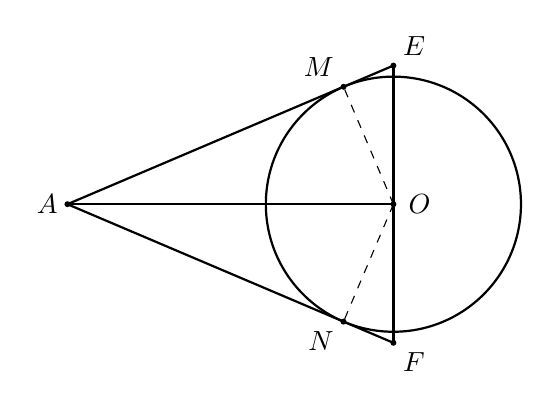
\begin{tikzpicture}[scale=0.9]
  \draw[thick] (0,0) circle (1.8);
  \coordinate (O) at (0,0);
  \coordinate (A) at (-4.6,0);
  \coordinate (M) at (-0.704,1.657);
  \coordinate (N) at (-0.704,-1.657);
  \coordinate (E) at (0,1.956);
  \coordinate (F) at (0,-1.956);
  \draw[thick] (A) -- (E);
  \draw[thick] (A) -- (F);
  \draw[thick] (A) -- (O);
  \draw[thick] (E) -- (F);
  \draw[dashed] (O) -- (M);
  \draw[dashed] (O) -- (N);
  \fill (O) circle (1.2pt) node[right=2pt] {$O$};
  \fill (A) circle (1.2pt) node[left] {$A$};
  \fill (M) circle (1.2pt) node[above left] {$M$};
  \fill (N) circle (1.2pt) node[below left] {$N$};
  \fill (E) circle (1.2pt) node[above right] {$E$};
  \fill (F) circle (1.2pt) node[below right] {$F$};
\end{tikzpicture}
\end{center}
\nopagebreak[4]
\Needspace{4\baselineskip}
\textbf{解析}

\Needspace{5\baselineskip}
连接 $OM\text{、}ON$。因为 $M\text{、}N$ 是切点，所以

\nopagebreak[4]
\[
OM\perp AE,
\qquad ON\perp AF.
\]

\Needspace{5\baselineskip}
在 $\mathrm{Rt}\triangle OMA$ 与 $\mathrm{Rt}\triangle ONA$ 中：$OA=OA$（公共斜边），$OM=ON$（圆的半径相等），所以

\nopagebreak[4]
\[
\mathrm{Rt}\triangle OMA\cong\mathrm{Rt}\triangle ONA
\quad\Longrightarrow\quad
\angle OAM=\angle OAN.
\]

\Needspace{5\baselineskip}
由于 $M$ 在 $AE$ 上、$N$ 在 $AF$ 上，即

\nopagebreak[4]
\[
\angle EAO=\angle FAO.
\]

\Needspace{5\baselineskip}
再看 $\mathrm{Rt}\triangle AOE$ 与 $\mathrm{Rt}\triangle AOF$：$OA=OA$（公共直角边），$\angle EAO=\angle FAO$（已证），加上直角相等，所以

\nopagebreak[4]
\[
\mathrm{Rt}\triangle AOE\cong\mathrm{Rt}\triangle AOF
\quad\Longrightarrow\quad
AE=AF
\]

（对应边相等）。
\nopagebreak[4]
\begin{center}% 1977 年广东卷第 6 题：AE、AF 切圆 O 于 M、N，直径 EF 过圆心 O 且垂直于 AO，
% OM、ON 画虚线（按源卷第 3 页布局）
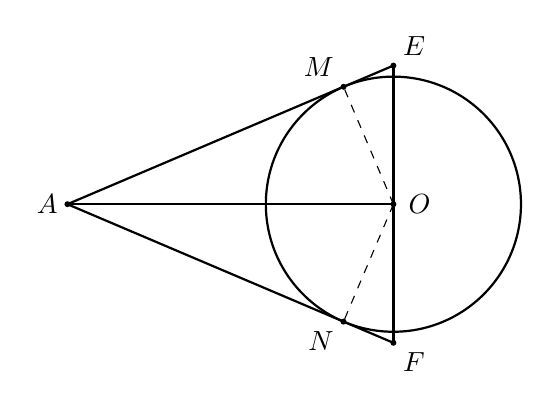
\begin{tikzpicture}[scale=0.9]
  \draw[thick] (0,0) circle (1.8);
  \coordinate (O) at (0,0);
  \coordinate (A) at (-4.6,0);
  \coordinate (M) at (-0.704,1.657);
  \coordinate (N) at (-0.704,-1.657);
  \coordinate (E) at (0,1.956);
  \coordinate (F) at (0,-1.956);
  \draw[thick] (A) -- (E);
  \draw[thick] (A) -- (F);
  \draw[thick] (A) -- (O);
  \draw[thick] (E) -- (F);
  \draw[dashed] (O) -- (M);
  \draw[dashed] (O) -- (N);
  \fill (O) circle (1.2pt) node[right=2pt] {$O$};
  \fill (A) circle (1.2pt) node[left] {$A$};
  \fill (M) circle (1.2pt) node[above left] {$M$};
  \fill (N) circle (1.2pt) node[below left] {$N$};
  \fill (E) circle (1.2pt) node[above right] {$E$};
  \fill (F) circle (1.2pt) node[below right] {$F$};
\end{tikzpicture}
\end{center}
\nopagebreak[4]
\gkanswer{答案：见解析版}

\end{answer}
\begin{answer}
\gksolhead{7}{}

\textbf{题目}：

如果平面内一动点 $P$ 到点 $(-4,\ 0)$ 的距离等于它到直线 $x=-\dfrac{25}{4}$ 的距离的 $\dfrac{4}{5}$，求 $P$ 点的轨迹方程，又这是一条什么曲线？

\Needspace{5\baselineskip}
\textbf{参考题 1．} 方程组

\nopagebreak[4]
\[
\begin{cases}
x_1+3x_2+2x_3-x_4=1,\\
x_2-2x_3+x_4=-1,\\
2x_1+x_3+2x_4=0,\\
2x_2+ax_3-2x_4=1
\end{cases}
\]

中，当 $a$ 取什么值时，该方程组有解？（有多少组解？）又当 $a$ 取什么值时，方程组无解？

\textbf{参考题 2．} 有一份印刷品，其排版面积（矩形）占 $432$ 平方厘米，它的两边都留有 $4$ 厘米宽的空白，顶部和底部留有 $3$ 厘米宽的空白。问应该如何选取纸张的尺寸，才能使纸的用量最少？

\begin{gktip}
原源 PDF 第 5 页附有纸张与排版面的示意图；LaTeX 版按源图重绘。
\end{gktip}
\nopagebreak[4]
\begin{center}% 1977 年广东卷参考题 2：纸张矩形（左右长 x、上下宽 y），内阴影矩形为排版面 432，
% 左右边距 4 厘米、上下边距 3 厘米（按源卷第 5 页布局）
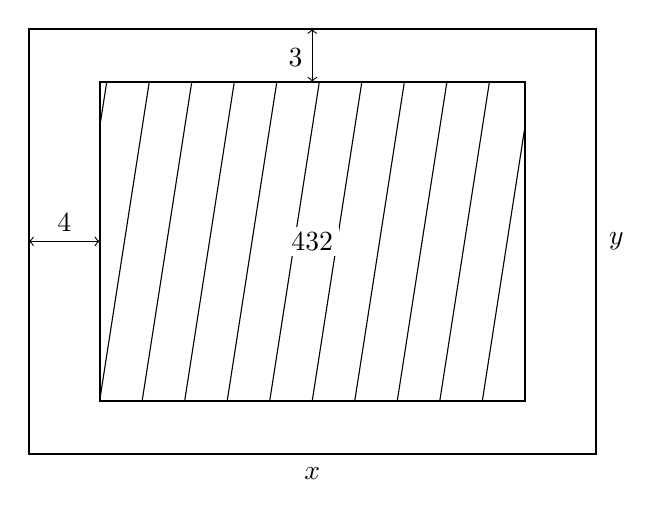
\begin{tikzpicture}[scale=0.9]
  \draw[thick] (0,0) rectangle (8,6);
  \begin{scope}
    \clip (1,0.75) rectangle (7,5.25);
    \foreach \i in {-7,...,10}
      \draw (1+\i*0.6,0.75) -- (1.7+\i*0.6,5.25);
  \end{scope}
  \draw[thick] (1,0.75) rectangle (7,5.25);
  \node[fill=white,inner sep=2pt] at (4,3) {$432$};
  % 边距标注
  \draw[<->] (0,3) -- (1,3);
  \node[above] at (0.5,3) {$4$};
  \draw[<->] (4,5.25) -- (4,6);
  \node[left] at (4,5.6) {$3$};
  % 纸张尺寸标注
  \node[below] at (4,-0.05) {$x$};
  \node[right] at (8.05,3) {$y$};
\end{tikzpicture}
\end{center}
\nopagebreak[4]
\Needspace{4\baselineskip}
\textbf{解析}

\Needspace{5\baselineskip}
设动点 $P$ 的坐标为 $(x,\ y)$。$P$ 到点 $(-4,\ 0)$ 的距离为

\nopagebreak[4]
\[
\sqrt{(x+4)^2+y^2},
\]

\Needspace{5\baselineskip}
$P$ 到直线 $x=-\dfrac{25}{4}$ 的距离为 $\left|x+\dfrac{25}{4}\right|$。依题意，

\nopagebreak[4]
\[
\sqrt{(x+4)^2+y^2}=\frac{4}{5}\left|x+\frac{25}{4}\right|.
\]

\Needspace{5\baselineskip}
两边平方：

\nopagebreak[4]
\[
(x+4)^2+y^2=\frac{16}{25}\left(x+\frac{25}{4}\right)^2,
\]

\nopagebreak[4]
\[
x^2+8x+16+y^2=\frac{16}{25}x^2+8x+25.
\]

\Needspace{5\baselineskip}
消去一次项，得

\nopagebreak[4]
\[
\frac{9}{25}x^2+y^2=9,
\]

\Needspace{5\baselineskip}
即

\nopagebreak[4]
\[
\frac{x^2}{25}+\frac{y^2}{9}=1.
\]

此轨迹是椭圆，其中 $a=5$、$b=3$、$c=\sqrt{25-9}=4$。它恰以 $(-4,\ 0)$ 为左焦点，直线 $x=-\dfrac{25}{4}=-\dfrac{a^2}{c}$ 为左准线，离心率 $e=\dfrac{c}{a}=\dfrac{4}{5}$，与椭圆的第二定义（动点到焦点的距离与到准线的距离之比为离心率）完全吻合。

\textbf{参考题 1}

记方程组的四个方程为（1）—（4）。

\Needspace{5\baselineskip}
\textbf{解法一（消元）}：（1）式 $\times 2-$（3）式消去 $x_1$，得

\nopagebreak[4]
\[
6x_2+3x_3-4x_4=2.
\qquad(5)
\]

\Needspace{5\baselineskip}
（2）式 $\times 6-$（5）式，得

\nopagebreak[4]
\[
-15x_3+10x_4=-8.
\qquad(6)
\]

\Needspace{5\baselineskip}
（2）式 $\times 2-$（4）式，得

\nopagebreak[4]
\[
-(a+4)x_3+4x_4=-3.
\qquad(7)
\]

\Needspace{5\baselineskip}
（6）式 $\times 2-$（7）式 $\times 5$，消去 $x_4$：

\nopagebreak[4]
\[
\bigl(5a-10\bigr)x_3=-1.
\]

当 $a\neq 2$ 时，$x_3=-\dfrac{1}{5(a-2)}$，随后可由（6）（7）式唯一地解出 $x_4$，再逐级回代唯一地求得 $x_1\text{、}x_2$，故原方程组有唯一一组解。

当 $a=2$ 时，（6）（7）两式为 $-15x_3+10x_4=-8$ 与 $-6x_3+4x_4=-3$。把第二式乘 $-\dfrac{5}{2}$ 得 $15x_3-10x_4=\dfrac{15}{2}$，与第一式相加得 $0=-\dfrac{1}{2}$，矛盾，故原方程组无解。

\Needspace{5\baselineskip}
\textbf{解法二（行列式）}：系数行列式按第一列展开：

\nopagebreak[4]
\[
|\Delta|=
\begin{vmatrix}
1 & 3 & 2 & -1\\
0 & 1 & -2 & 1\\
2 & 0 & 1 & 2\\
0 & 2 & a & -2
\end{vmatrix}
=
\begin{vmatrix}
1 & -2 & 1\\
0 & 1 & 2\\
2 & a & -2
\end{vmatrix}
+2\begin{vmatrix}
3 & 2 & -1\\
1 & -2 & 1\\
2 & a & -2
\end{vmatrix}.
\]

\Needspace{5\baselineskip}
分别计算两个三阶行列式：

\nopagebreak[4]
\[
\begin{vmatrix}
1 & -2 & 1\\
0 & 1 & 2\\
2 & a & -2
\end{vmatrix}
=-12-2a,
\qquad
\begin{vmatrix}
3 & 2 & -1\\
1 & -2 & 1\\
2 & a & -2
\end{vmatrix}
=16-4a.
\]

\Needspace{5\baselineskip}
于是

\nopagebreak[4]
\[
|\Delta|=(-12-2a)+2(16-4a)=10(2-a).
\]

当 $a\neq 2$ 时，$|\Delta|\neq 0$，原方程组有唯一一组解；当 $a=2$ 时，$|\Delta|=0$，与解法一的结果相同，原方程组无解。

\textbf{参考题 2}

\Needspace{5\baselineskip}
设纸张左右长 $x$ 厘米、上下宽 $y$ 厘米，纸面积为 $S$ 平方厘米。左右各留 $4$ 厘米、上下各留 $3$ 厘米后，排版面积为

\nopagebreak[4]
\[
(x-8)(y-6)=432.
\qquad(1)
\]

\nopagebreak[4]
\[
S=xy.
\qquad(2)
\]

\Needspace{5\baselineskip}
由（1）得 $y=\dfrac{432}{x-8}+6$（$x>8$），代入（2）：

\nopagebreak[4]
\[
S=\frac{432x}{x-8}+6x
=432+\frac{3456}{x-8}+6x
=\frac{3456}{x-8}+6(x-8)+480.
\]

\Needspace{5\baselineskip}
由均值不等式（两项均为正），

\nopagebreak[4]
\[
S\geq 2\sqrt{\frac{3456}{x-8}\cdot 6(x-8)}+480
=2\sqrt{3456\times 6}+480
=2\times 144+480
=768,
\]

\Needspace{5\baselineskip}
等号当且仅当

\nopagebreak[4]
\[
\frac{3456}{x-8}=6(x-8)
\quad\Longrightarrow\quad
(x-8)^2=576
\quad\Longrightarrow\quad
x_1=32,\quad x_2=-16\ (\text{\text{舍去}})
\]

\Needspace{5\baselineskip}
时成立。此时

\nopagebreak[4]
\[
y=\frac{432}{32-8}+6=18+6=24\ (\text{\text{厘米}}).
\]

即选取左右长 $32$ 厘米、上下宽 $24$ 厘米的纸张时，用纸最少，最小面积为 $768$ 平方厘米。
\nopagebreak[4]
\begin{center}% 1977 年广东卷参考题 2：纸张矩形（左右长 x、上下宽 y），内阴影矩形为排版面 432，
% 左右边距 4 厘米、上下边距 3 厘米（按源卷第 5 页布局）
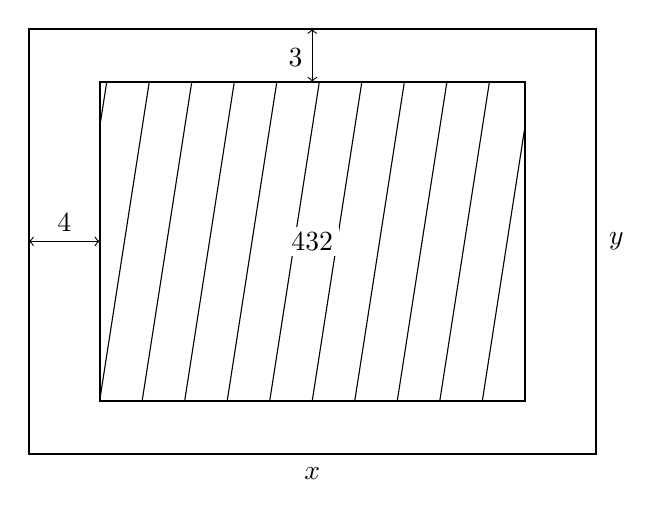
\begin{tikzpicture}[scale=0.9]
  \draw[thick] (0,0) rectangle (8,6);
  \begin{scope}
    \clip (1,0.75) rectangle (7,5.25);
    \foreach \i in {-7,...,10}
      \draw (1+\i*0.6,0.75) -- (1.7+\i*0.6,5.25);
  \end{scope}
  \draw[thick] (1,0.75) rectangle (7,5.25);
  \node[fill=white,inner sep=2pt] at (4,3) {$432$};
  % 边距标注
  \draw[<->] (0,3) -- (1,3);
  \node[above] at (0.5,3) {$4$};
  \draw[<->] (4,5.25) -- (4,6);
  \node[left] at (4,5.6) {$3$};
  % 纸张尺寸标注
  \node[below] at (4,-0.05) {$x$};
  \node[right] at (8.05,3) {$y$};
\end{tikzpicture}
\end{center}
\nopagebreak[4]
\gkanswer{答案：$\dfrac{x^2}{25}+\dfrac{y^2}{9}=1$，轨迹是椭圆。}

\end{answer}